% TikZ Asset: FA22GraphTheoryBipartiteMatchingsTikZ-001
%
% Asset ID: FA22GraphTheoryBipartiteMatchingsTikZ-001
% Topic ID: FA22GraphTheoryBipartiteMatchings
% Unit: FA22
% Topic code: FA22-GRAPH
% Related lesson file: FA22_graph_theory_bipartite_matchings_lesson.md
% Related lesson section: Section 9.5 Printable TikZ Matching Diagram
%
% Used placeholder:
% [VISUAL PLACEHOLDER: FA22GraphTheoryBipartiteMatchingsTikZ-001 | Source: CCEA FA22-GRAPH-LO003 | Insert from tikz/FA22GraphTheoryBipartiteMatchingsTikZ-001.tex | Purpose: Provide a precise mathematical diagram of a bipartite graph and complete matching for printable notes.]
%
% Source:
% CCEA FA22-GRAPH-LO003
%
% Purpose:
% Provide a precise mathematical diagram of a bipartite graph and complete matching.
%
% Creation notes:
% This diagram shows a bipartite graph with U = {A, B, C} and W = {1, 2, 3}.
% All allowed edges are shown, while the complete matching
% M = {(A,2), (B,1), (C,3)}
% is highlighted.
%
% Off-spec guard:
% This diagram does not show a weighted cost matrix, Hungarian algorithm,
% row reduction, column reduction, dummy entries or maximum allocation.

\documentclass[tikz,border=10pt]{standalone}

\usepackage{xcolor}
\usepackage{amsmath}
\usetikzlibrary{positioning,fit,backgrounds}

\definecolor{Canvas}{HTML}{FAF9F6}
\definecolor{Panel}{HTML}{FFFFF0}
\definecolor{Divider}{HTML}{E5E5EA}
\definecolor{AccentGold}{HTML}{D4AF37}
\definecolor{AccentSoftGold}{HTML}{C5A059}
\definecolor{AccentBlush}{HTML}{FBEFEF}
\definecolor{TextColor}{HTML}{2C2C2E}
\definecolor{MutedLine}{HTML}{A9A9B2}

\begin{document}

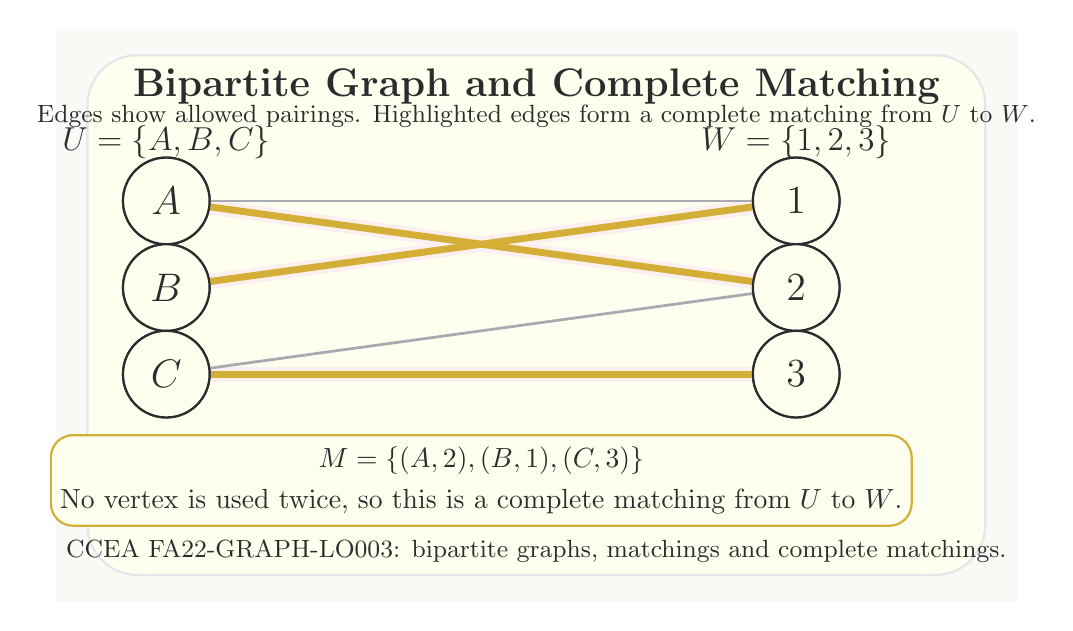
\begin{tikzpicture}[
    vertex/.style={circle, draw=TextColor, fill=Panel, line width=0.8pt, minimum size=11mm, font=\Large\bfseries, text=TextColor},
    setlabel/.style={font=\large\bfseries, text=TextColor},
    smallnote/.style={font=\small, text=TextColor, align=center},
    allowededge/.style={draw=MutedLine, line width=1.0pt},
    matchedge/.style={draw=AccentGold, line width=2.5pt},
    glowedge/.style={draw=AccentBlush, line width=5.5pt},
    setbox/.style={draw=AccentSoftGold, dashed, rounded corners=18pt, line width=0.8pt},
    notebox/.style={draw=AccentGold, fill=Panel, rounded corners=8pt, line width=0.8pt}
]

\fill[Canvas] (-1.4,-4.0) rectangle (10.8,3.3);
\draw[draw=Divider, fill=Panel, rounded corners=18pt, line width=0.8pt] (-1.0,-3.65) rectangle (10.4,2.95);

\node[font=\Large\bfseries, text=TextColor] at (4.7,2.55) {Bipartite Graph and Complete Matching};
\node[smallnote] at (4.7,2.18) {Edges show allowed pairings. Highlighted edges form a complete matching from \(U\) to \(W\).};

\node[vertex] (A) at (0,1.1) {$A$};
\node[vertex] (B) at (0,0) {$B$};
\node[vertex] (C) at (0,-1.1) {$C$};

\node[vertex] (one) at (8,1.1) {$1$};
\node[vertex] (two) at (8,0) {$2$};
\node[vertex] (three) at (8,-1.1) {$3$};

\node[setlabel] at (0,1.85) {$U=\{A,B,C\}$};
\node[setlabel] at (8,1.85) {$W=\{1,2,3\}$};

\begin{scope}[on background layer]
    \node[setbox, fit=(A)(B)(C), inner xsep=12pt, inner ysep=14pt] {};
    \node[setbox, fit=(one)(two)(three), inner xsep=12pt, inner ysep=14pt] {};
\end{scope}

\draw[glowedge] (A) -- (two);
\draw[glowedge] (B) -- (one);
\draw[glowedge] (C) -- (three);

\draw[allowededge] (A) -- (one);
\draw[allowededge] (C) -- (two);

\draw[matchedge] (A) -- (two);
\draw[matchedge] (B) -- (one);
\draw[matchedge] (C) -- (three);

\node[vertex] at (A) {$A$};
\node[vertex] at (B) {$B$};
\node[vertex] at (C) {$C$};
\node[vertex] at (one) {$1$};
\node[vertex] at (two) {$2$};
\node[vertex] at (three) {$3$};

\node[notebox, align=center, text=TextColor, minimum width=7.5cm, minimum height=1.15cm] at (4,-2.45)
      {\(\displaystyle M=\{(A,2),(B,1),(C,3)\}\)\\[3pt]
       No vertex is used twice, so this is a complete matching from \(U\) to \(W\).};

\node[smallnote] at (4.7,-3.35) {CCEA FA22-GRAPH-LO003: bipartite graphs, matchings and complete matchings.};

\end{tikzpicture}

\end{document}
